%%%%%%%%%%%%%%%%%%%%%%%%%%%%%%%%%%%%%%%%%%%%%%%%%%%%%%%%%%%%%%
% --> INTRODUCCIÓN
%%%%%%%%%%%%%%%%%%%%%%%%%%%%%%%%%%%%%%%%%%%%%%%%%%%%%%%%%%%%%%
\section{Introducción}

Según \cite{R1}, la programación genérica está mucho más centrada en los algoritmos que en los datos, y su postulado fundamental puede sintetizarse en una palabra: generalización. Significa que, en la medida de lo posible, los algoritmos deben ser parametrizados al máximo y expresados de la forma más independiente posible de detalles concretos, permitiendo así que puedan servir para la mayor variedad posible de tipos y estructuras de datos.

Un patrón o plantilla es una forma de objeto, que se aplica a diferentes instancias, sin especificar el tipo de objeto a ser referenciado. El patrón con un simple código cubre un gran rango de funciones de
sobrecarga denominadas funciones patrones o un gran rango de clases denominadas clases patrones \cite{R2}.

Por ejemplo, para realizar una operación con \texttt{int}, \texttt{double} y \texttt{char}, se puede hacer sobrecargando la función \texttt{max} como se muestra a continuación:

\begin{minted}[linenos,autogobble,bgcolor=bg,breaklines,fontsize=\footnotesize ]{c++}
int max(int a,int b)
{
 return a>b?a:b;
}
double max(double a,double b)
{
 return a>b?a:b;
}
char max(char a,char b)
{
 return a>b?a:b;
}
\end{minted}

Pero haciendo uso de \texttt{template}, simplemente se puede hacer de la siguiente manera:

\begin{minted}[linenos,autogobble,bgcolor=bg,breaklines,fontsize=\footnotesize ]{c++}
template<class T>
T max(T a,T b)
{
 return a>b?a:b;
}
\end{minted}

%%%%%%%%%%%%%%%%%%%%%%%%%%%%%%%%%%%%%%%%%%%%%%%%%%%%%%%%%%%%%%
% --> OBJETIVOS
%%%%%%%%%%%%%%%%%%%%%%%%%%%%%%%%%%%%%%%%%%%%%%%%%%%%%%%%%%%%%%
\subsection{Objetivos}

A continuación, se enlistan los objetivos de este laboratorio.

%%%%%%%%%%%%%%%%%%%%%%%%%%%%%%%%%%%%%%%%%%%%%%%%%%%%%%%%%%%%%%
% --> OBJETIVO GENERAL
%%%%%%%%%%%%%%%%%%%%%%%%%%%%%%%%%%%%%%%%%%%%%%%%%%%%%%%%%%%%%%
\subsubsection{Objetivo General}
\begin{itemize}
\item Diseñar una serie de clases con plantillas que permitan hacer operaciones básicas con enteros. reales, fracciones, polinomios y matrices.
\end{itemize}

%%%%%%%%%%%%%%%%%%%%%%%%%%%%%%%%%%%%%%%%%%%%%%%%%%%%%%%%%%%%%%
% --> OBJETIVOS ESPECÍFICOS
%%%%%%%%%%%%%%%%%%%%%%%%%%%%%%%%%%%%%%%%%%%%%%%%%%%%%%%%%%%%%%
\subsubsection{Objetivos Específicos}
\begin{itemize}
\item Implementar una clase para realizar operaciones básicas con fracciones.
\item Implementar una clase para realizar operaciones básicas con matrices.
\item Implementar una clase para realizar operaciones básicas con polinomios.
\item Desarrollar una clase emplantilla para que logre operar con diferentes tipos de datos de entrada.
\item Verificar las clases desarrolladas en un programa principal.
\end{itemize}

%%%%%%%%%%%%%%%%%%%%%%%%%%%%%%%%%%%%%%%%%%%%%%%%%%%%%%%%%%%%%%
% --> ENUNCIADO
%%%%%%%%%%%%%%%%%%%%%%%%%%%%%%%%%%%%%%%%%%%%%%%%%%%%%%%%%%%%%%
\newpage

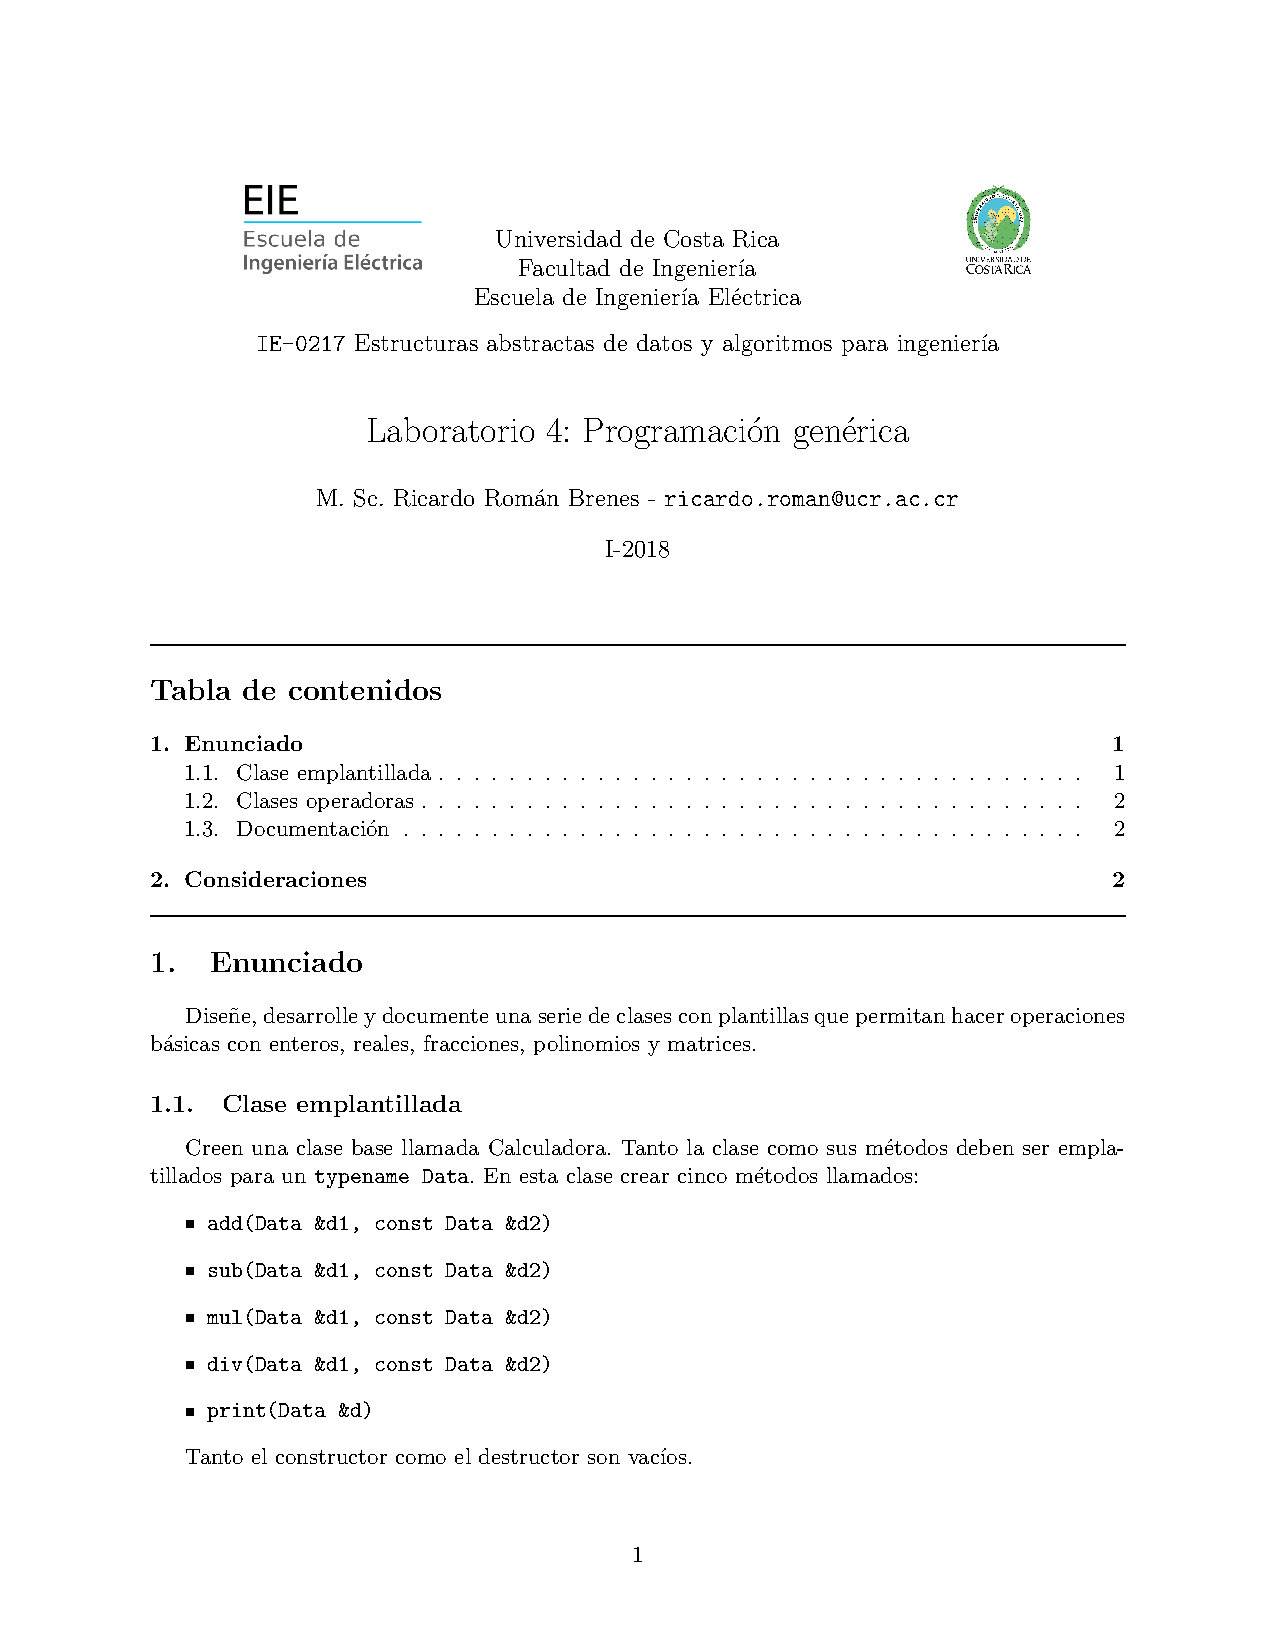
\includepdf[pages=1,pagecommand=\section{Enunciado}, scale=0.8]{enunciados/enun4} 
\includepdf[pages=2,pagecommand={},scale=0.8]{enunciados/enun4}

%%%%%%%%%%%%%%%%%%%%%%%%%%%%%%%%%%%%%%%%%%%%%%%%%%%%%%%%%%%%%%
% --> SOLUCIÓN
%%%%%%%%%%%%%%%%%%%%%%%%%%%%%%%%%%%%%%%%%%%%%%%%%%%%%%%%%%%%%%
\section{Solución}

%%%%%%%%%%%%%%%%%%%%%%%%%%%%%%%%%%%%%%%%%%%%%%%%%%%%%%%%%%%%%%
% --> CLASE POLINOMIO
%%%%%%%%%%%%%%%%%%%%%%%%%%%%%%%%%%%%%%%%%%%%%%%%%%%%%%%%%%%%%%
\subsection{Clase Polinomio}

La clase \texttt{Polynomial} realiza operaciones básicas de polinomios de grado n. En este archivo \texttt{.h} se declaran todas las funciones necesarias, así como dos variables necesarias para la ejecución, una tipo \texttt{int} para almacenar el tamaño del polinomio, es decir, la cantidad de coeficientes que posee. Y otra variable tipo \texttt{double*} para almacenar estos coeficientes, esto es un puntero que básicamente funciona como un \texttt{array}.

\begin{minted}[linenos,autogobble,bgcolor=bg,breaklines,fontsize=\footnotesize ]{c++}
class Polynomial
{
	public:
		Polynomial(int Grado,double Coeficientes[]);
		Polynomial(const Polynomial &l_cCopyPolynomial);
		~Polynomial();
		Polynomial operator+(const Polynomial &P);
		Polynomial operator-(const Polynomial &P);
		Polynomial operator*(const Polynomial &P);
		Polynomial operator/(const Polynomial &P);
		void operator~(void);
	protected:
		double* m_pCoefPolinomio;
	private:
		int m_iTamPolinomio;

};

\end{minted}

\subsubsection{Métodos de \texttt{Polynomial}.}
\begin{itemize}
    \item \textbf{Método constructor:}
    
    El método constructor por defecto requiere de dos argumentos, uno es el grado del polinomio, y el otro es un arreglo del tipo \texttt{double} con los coeficientes que conforman el polinomio. Haciendo uso de un ciclo \texttt{for} se almacenan los coeficientes en los atributos del objeto creado. Además se reserva memoria para este arreglo en donde se van a guardar los coeficientes.
    
    \begin{minted}[linenos,autogobble,bgcolor=bg,breaklines,fontsize=\footnotesize ]{c++}
    Polynomial::Polynomial(int l_iGrado, double l_pCoef []){
  cout << endl << "Creando polinomio." << endl;
  this->m_iTamPolinomio = l_iGrado+1;
  this->m_pCoefPolinomio = new double[l_iGrado+1];
  cout << endl << "Polinomio: ";
  for (int i = 0; i < this->m_iTamPolinomio; i++) {
    if (i == this->m_iTamPolinomio-1){
      this->m_pCoefPolinomio[i] = l_pCoef[i];
      cout << this->m_pCoefPolinomio[i] << "x^" << l_iGrado << endl;
    }
    else{
      this->m_pCoefPolinomio[i] = l_pCoef[i];
      cout << this->m_pCoefPolinomio[i] << "x^" << l_iGrado << " +";
      l_iGrado--;
    }
  }
  cout << endl << endl;
}
    \end{minted}
    
    \item \textbf{Método constructor por copia:}
    
    El constructor por copia crea una copia de un objeto del tipo \texttt{Polynomial}, esto será de utilidad cuando se realicen las operaciones y se necesite guardar el resultado en un nuevo objeto.
    \begin{minted}[linenos,autogobble,bgcolor=bg,breaklines,fontsize=\footnotesize ]{c++}
Polynomial::Polynomial(const Polynomial &l_cCopyPolynomial){
  this->m_iTamPolinomio = l_cCopyPolynomial.m_iTamPolinomio;
  this->m_pCoefPolinomio = new double [l_cCopyPolynomial.m_iTamPolinomio];
  for (int h = 0; h < l_cCopyPolynomial.m_iTamPolinomio; h++) {
    this->m_pCoefPolinomio[h] = l_cCopyPolynomial.m_pCoefPolinomio[h];
  }
}
    \end{minted}
    
    \item \textbf{Método destructor:}
    
    El método destructor elimina la memoria utilizada en la creación del objeto, además libera la memoria reservada por el comando \texttt{new} utilizado anteriormente.
    
    \begin{minted}[linenos,autogobble,bgcolor=bg,breaklines,fontsize=\footnotesize ]{c++}
    Polynomial::~Polynomial(){
    delete[] this->m_pCoefPolinomio;
    }
    \end{minted}
    
    \item \textbf{Sobrecarga de operadores +, -:}
    
    Estos métodos sobrecargan los operadores para poder realizar las operaciones entre polinomios, el algoritmo utilizado es básicamente el mismo en los cuatro casos.
    
    Se recibe como argumente un polinomio y se compara los tamaños de estos dos objetos, en donde se guarda la diferencia en una variable tipo \texttt{int}. Posteriormente se inicializa un arreglo de tipo \texttt{double} del tamaño del polinomio más grande. Se debe mencionar que los arreglos de los coeficientes deben estar en orden decreciente, de tal manera de que si se tiene un polinomio $P(x)=2x^4+5.8x^2+6$ se tiene, por ejemplo, un arreglo de la forma [ 2  0  5.8  0  6 ]. Una vez listo lo anterior, se almacenan los valores del polinomio mayor desde cero hasta la diferencia calculada entre los tamaños. Luego, se recorren las demás casillas, en donde sí se debe realizar la operación necesaria, de igual manera se almacenan los valores. Finalmente, se crea un nuevo objeto tipo polinomio con los resultados que se retorna. Para el caso de la resta se utiliza el mismo código, pero se cambia el símbolo de la operación.
    
    \begin{minted}[linenos,autogobble,bgcolor=bg,breaklines,fontsize=\footnotesize ]{c++}
Polynomial Polynomial::operator+(const Polynomial &P){
  if (this->m_iTamPolinomio > P.m_iTamPolinomio){
    int l_iDifGrados = this->m_iTamPolinomio - P.m_iTamPolinomio;
    double l_pSuma [this->m_iTamPolinomio];
    for (int q = 0; q < l_iDifGrados; q++) {
      l_pSuma[q] = this->m_pCoefPolinomio[q];
    }
    for (int w = l_iDifGrados; w < this->m_iTamPolinomio; w++) {
      l_pSuma[w] = this->m_pCoefPolinomio[w] + P.m_pCoefPolinomio[w-l_iDifGrados];
    }
    Polynomial Suma(m_iTamPolinomio-1,l_pSuma);
    return Suma;
  }
  else {
    int l_iDifGrados = P.m_iTamPolinomio - this->m_iTamPolinomio;
    double l_pSuma [P.m_iTamPolinomio];
    for (int q = 0; q < l_iDifGrados; q++) {
      l_pSuma[q] = P.m_pCoefPolinomio[q];
    }
    for (int w = l_iDifGrados; w < P.m_iTamPolinomio; w++) {
      l_pSuma[w] = this->m_pCoefPolinomio[w-l_iDifGrados] + P.m_pCoefPolinomio[w];
    }
    Polynomial Suma(P.m_iTamPolinomio-1,l_pSuma);
    return Suma;
  }
}
    \end{minted}
    
    \item \textbf{Sobrecarga del operador *:}
    
    La multiplicación de polinomios no se realiza entrada por entrada como la suma y la resta, por esto se utiliza un algoritmo distinto. Se sabe que si se tienen dos polinomios de grado $a$ y $b$, el grado del resultado de su multiplicación es $a+b-1$. Se parte del principio anterior para crear un arreglo del tamaño necesario para el resultado. Además, se inicializan todas las casillas de este arreglo con un valor de cero. Una vez que se tiene esto, se procede a recorrer los dos arreglos que contienen los coeficientes de los polinomios, aquí se multiplican todas las casillas entre sí, pero a la vez se le va sumando el valor que se almacena con cada iteración en una casilla determinada. Así se realiza correctamente la multiplicación, en donde primero se multiplican todos los términos, y luego se suman los semejantes.
    
    \begin{minted}[linenos,autogobble,bgcolor=bg,breaklines,fontsize=\footnotesize ]{c++}
Polynomial Polynomial::operator*(const Polynomial &P){
  double l_pMult [this->m_iTamPolinomio+P.m_iTamPolinomio-1];
  for(int x = 0; x < this->m_iTamPolinomio+P.m_iTamPolinomio-1; x++){
    l_pMult[x] = 0;
  }
  for (int c = 0; c < this->m_iTamPolinomio; c++) {
    for (int t = 0; t < P.m_iTamPolinomio; t++){
      l_pMult[c + t] = l_pMult[c + t] + this->m_pCoefPolinomio[c]*P.m_pCoefPolinomio[t];
    }
  }
  Polynomial Mult(this->m_iTamPolinomio+P.m_iTamPolinomio-2,l_pMult);
  return Mult;
}
    \end{minted}
    
\end{itemize}

%%%%%%%%%%%%%%%%%%%%%%%%%%%%%%%%%%%%%%%%%%%%%%%%%%%%%%%%%%%%%%
% --> CLASE FRACCIÓN
%%%%%%%%%%%%%%%%%%%%%%%%%%%%%%%%%%%%%%%%%%%%%%%%%%%%%%%%%%%%%%
\subsection{Clase Fracción}

En la clase \texttt{Fraction}, se crean los métodos necesarios para efectuar operaciones básicas con fracciones. Los elementos de tipo \texttt{Fraction} contienen simplemente dos atributos: numerador y denominador. En este caso, estos valores solo pueden ser de tipo entero, dado que no tiene sentido la idea de fracciones con cuyo numerador y/o denominador sea un número decimal. Además, no se permite que el denominador sea 0.

\begin{minted}[linenos,autogobble,bgcolor=bg,breaklines,fontsize=\footnotesize ]{c++}
class Fraction
{
	public:
		Fraction  ();
		Fraction  (int l_iNum, int l_iDen);
		Fraction  (const Fraction &l_cCopyFraction);
		~Fraction ();
		Fraction  operator+(const Fraction &rhs);
		Fraction  operator-(const Fraction &rhs);
		Fraction  operator*(const Fraction &rhs);
		Fraction  operator/(const Fraction &rhs);
		void      operator~();
	protected:
	private:
		int       m_iNumerador;
		int       m_iDenominador;
		void      checkDen();
};
\end{minted}


\subsubsection{Métodos de \texttt{Fraction}.}
\begin{itemize}
    \item \textbf{Método constructor vacío:} Aunque existe un constructor vacío, no se permite la existencia de un elemento de tipo \texttt{Fraction} sin asignar sus elementos. Por esto, este método pide ingresar los valores.
    
    
        \begin{minted}[linenos,autogobble,bgcolor=bg,breaklines,fontsize=\footnotesize ]{c++}
        Fraction::Fraction(){
            cout << endl << "Creando nueva fracción..." << endl << "Ingrese el numerador: " << endl << endl;
            cin >> this->m_iNumerador;
            checkDen();
        };
        \end{minted}

    \item \textbf{Método \texttt{checkDen()}:} Es un método para asignar el denominador. Pide el valor al usuario y lo asigna a una variable temporal. Revisa si el valor es igual a 0, si lo es, lo vuelve a solicitar; si no, lo asigna al atributo del elemento.
        \begin{minted}[linenos,autogobble,bgcolor=bg,breaklines,fontsize=\footnotesize ]{c++}
        void Fraction::checkDen(){
            int l_itmp = 0;
            bool l_bDiv0 = false;
            do {
                cout << "Ingrese el denominador: " << endl << endl;
                cin >> l_itmp;
                if (l_itmp == 0){
                    l_bDiv0 = true;
                    cout << endl << "---ERROR: El denominador NO puede ser 0---" << endl << endl;
                }
                else {
                    this->m_iDenominador = l_itmp;
                    l_bDiv0 = false;
                }
            } while (l_bDiv0 == true);
        }
        \end{minted}
    
    \item \textbf{Método constructor con parámetros:} Inicializa los atributos con los valores pasados como parámetros. Se usa \texttt{checkDen()} en caso de que se intente crear una fracción con denominador 0.
        \begin{minted}[linenos,autogobble,bgcolor=bg,breaklines,fontsize=\footnotesize ]{c++}
        Fraction::Fraction(int l_iNum, int l_iDen){
            this->m_iNumerador=l_iNum;
            if (l_iDen != 0){
                this->m_iDenominador = l_iDen;
            }
            else{
                cout << endl << "---ERROR: El denominador NO puede ser 0---" << endl << endl;
                checkDen();
            }
        }
        \end{minted}
        
    \item \textbf{Método constructor por copia:} Simplementa asigna al elemento creado los atributos del elemento pasado por referencia.
        \begin{minted}[linenos,autogobble,bgcolor=bg,breaklines,fontsize=\footnotesize ]{c++}
        Fraction::Fraction(const Fraction &l_cCopyFraction){
            this->m_iNumerador = l_cCopyFraction.m_iNumerador;
            this->m_iDenominador = l_cCopyFraction.m_iDenominador;
        }
        \end{minted}
        
    \item \textbf{Sobrecarga de operadores + y -: } Implementan la suma y resta sencilla de fracciones. 
        \begin{minted}[linenos,autogobble,bgcolor=bg,breaklines,fontsize=\footnotesize ]{c++}
        Fraction Fraction::operator+(const Fraction &rhs){
            int l_iNuevoNum = (this->m_iNumerador*rhs.m_iDenominador)+(this->m_iDenominador*rhs.m_iNumerador);
            int l_iNuevoDen = (this->m_iDenominador*rhs.m_iDenominador);
            Fraction suma(l_iNuevoNum,l_iNuevoDen);
            return suma;
        }
        
        Fraction Fraction::operator+(const Fraction &rhs){
            int l_iNuevoNum = (this->m_iNumerador*rhs.m_iDenominador)-(this->m_iDenominador*rhs.m_iNumerador);
            int l_iNuevoDen = (this->m_iDenominador*rhs.m_iDenominador);
            Fraction resta(l_iNuevoNum,l_iNuevoDen);
            return resta;
        }
        
        \end{minted}
    \item \textbf{Sobrecarga de operadores * y /: } Implementan la multiplicación y división de fracciones. El caso de la multiplicación es trivial. En el caso de la división, se debe prevenir la división entre 0. Para esto, se revisa si el numerador del elemento que actuará como divisor es 0, ya que ninguno de los denominadores podría serlo. Una limitación de este método es que, dado que el método debe retornar algo y para evitar errores de compilación o ejecución, en caso se que se intente dividir entre una fracción que es 0, la operación no se realiza y en su lugar simplemente se retorna una fracción unitaria.
    
    \begin{minted}[linenos,autogobble,bgcolor=bg,breaklines,fontsize=\footnotesize ]{c++}
    Fraction Fraction::operator*(const Fraction &rhs){
        int l_iNuevoNum = (this->m_iNumerador*rhs.m_iNumerador);
        int l_iNuevoDen = (this->m_iDenominador*rhs.m_iDenominador);
        Fraction mult(l_iNuevoNum,l_iNuevoDen);
        return mult;
    }
    
    Fraction Fraction::operator/(const Fraction &rhs){
        if (rhs.m_iNumerador != 0){
            int l_iNuevoNum = (this->m_iNumerador*rhs.m_iDenominador);
            int l_iNuevoDen = (this->m_iDenominador*rhs.m_iNumerador);
            Fraction div(l_iNuevoNum,l_iNuevoDen);
            return div;
        }
        else {
            cout << endl << "---ERROR: no se puede dividir entre cero---" << endl  << "Se le asignará a la fracción creada el valor 1" << endl;
            Fraction div(1,1);
            return div;
        }
    }
    
    \end{minted}
    
    \item \textbf{Sobrecarga del operador ~: } Imprime la fracción. Esto lo hace imprimiendo el numerador, seguido del caracter ``/'' y el denominador. 
    
    \begin{minted}[linenos,autogobble,bgcolor=bg,breaklines,fontsize=\footnotesize ]{c++}
    void Fraction::operator~(){
        if (this->m_iNumerador == 0){
            cout << this->m_iNumerador<< endl << endl;
        }
        else {
            cout << this->m_iNumerador << "/" << this->m_iDenominador  <<endl << endl;
        }
    }
    \end{minted}    
    
\end{itemize}

%%%%%%%%%%%%%%%%%%%%%%%%%%%%%%%%%%%%%%%%%%%%%%%%%%%%%%%%%%%%%%
% --> CLASE MATRIZ
%%%%%%%%%%%%%%%%%%%%%%%%%%%%%%%%%%%%%%%%%%%%%%%%%%%%%%%%%%%%%%
\subsection{Clase Matriz}

La clase \texttt{Matrix} realiza operaciones básicas de matrices. En la definición de la clase se declaran los métodos para realizar las operaciones básicas entre matrices, además de otros métodos adicionales para obtener las dimensiones de la matriz, así como poner y sacar valores de la matriz. Contiene tres atributos, un puntero en donde se guardar los valores de la matriz y dos variables que guardan la dimensión de la matriz.


\begin{minted}[linenos,autogobble,bgcolor=bg,breaklines,fontsize=\footnotesize ]{c++}
class Matrix
{
	public:
		Matrix  (int l_iRowSize, int l_iColSize, bool l_bFlag);
		Matrix	(double* l_pMatrix, int l_iRowSize, int l_iColSize);
		Matrix	(const Matrix &l_cCopyMat);
		~Matrix	();
		Matrix 	operator+(const Matrix &rhs);
		Matrix 	operator-(const Matrix &rhs);
		Matrix 	operator*(const Matrix &rhs);
		Matrix 	operator/(const Matrix &rhs);
		int 	GetRowSize();
		int 	GetColsSize();
		double 	GetMatValue(int l_iRow, int l_iCol);
		void  	SetMatValue(int l_iRC, double l_dValue);
		void 	operator~(void);
	protected:
	private:
		double* m_pMatrix;
		int 	m_iRows;
		int 	m_iCols;
};
\end{minted}

\subsubsection{Métodos de \texttt{Matrix}.}
\begin{itemize}
    \item \textbf{Método constructor:} genera una matriz con las dimensiones deseadas.
    
    \begin{minted}[linenos,autogobble,bgcolor=bg,breaklines,fontsize=\footnotesize ]{c++}
    Matrix::Matrix(int l_iRowSize, int l_iColSize, bool l_bFlag)
    {
      // Inicializa los valores
      this->m_iRows = l_iRowSize;
      this->m_iCols = l_iColSize;
      // Reserva memoria para la matriz
      this->m_pMatrix = new double[l_iRowSize*l_iColSize];
    
      // Si la bandera esta en alto, solicita los valores de la matriz al usuario,
      // sino solo crea la matrix con valores nulos
      if (l_bFlag)
      {
        int j = 0, k = 0;
        for(int i = 0; i <l_iRowSize*l_iColSize; i++)
        {
          cout << endl <<"Ingrese valor de la posición (" << k+1<<","<<j+1<<") : ";
          cin >> this->m_pMatrix[i];
          j++;
          if (j == l_iColSize)
          {
            j = 0;
            k++;
          }
        }
      }
      else
      {
        for(int i = 0; i <l_iRowSize*l_iColSize; i++) this->m_pMatrix[i] = 0.0;
      }
    }
    \end{minted}

    \item \textbf{Método constructor por copia:} genera una matriz con las dimensiones deseadas con un constructor por copia.
    
    \begin{minted}[linenos,autogobble,bgcolor=bg,breaklines,fontsize=\footnotesize ]{c++}
    Matrix::Matrix(const Matrix &l_cCopyMat)
    {
      this->m_iRows = l_cCopyMat.m_iRows;
      this->m_iCols = l_cCopyMat.m_iCols;
      this->m_pMatrix = new double[l_cCopyMat.m_iRows*l_cCopyMat.m_iCols];
    
      for(int i = 0; i <l_cCopyMat.m_iRows*l_cCopyMat.m_iCols; i++)
          this->m_pMatrix[i] = l_cCopyMat.m_pMatrix[i];
    }
    \end{minted}
    
    
    \item \textbf{Método destructor:} libera el espacio reservado por el arreglo de la matriz. 
    
    \begin{minted}[linenos,autogobble,bgcolor=bg,breaklines,fontsize=\footnotesize ]{c++}
    Matrix::~Matrix()
    {
      //cout << "Destruyendo Matrix" << endl ;
      delete[] m_pMatrix;
    }
    \end{minted}
    
    \item \textbf{operator$+$:} realiza la suma de matrices verificando que tengan las mismas dimensiones, sino es así devuelve una matriz con valores nulos. 
    
    \begin{minted}[linenos,autogobble,bgcolor=bg,breaklines,fontsize=\footnotesize ]{c++}
    Matrix Matrix::operator+(const Matrix &rhs)
    {
      Matrix l_mxResult(this->m_iRows,this->m_iCols,false);
    
      if(this->m_iRows == rhs.m_iRows && this->m_iCols == rhs.m_iCols)
      {
        for (int i = 0; i < this->m_iRows*this->m_iCols; i++)
          l_mxResult.SetMatValue(i,this->m_pMatrix[i] + rhs.m_pMatrix[i]);
      }
      else cout << "---ERROR: Operación suma no válida---" << '\n';
    
      return l_mxResult;
    }

    \end{minted}
    
    \item \textbf{operator-:} realiza la resta de matrices verificando que tengan las mismas dimensiones, sino es así devuelve una matriz con valores nulos. 
    
    \begin{minted}[linenos,autogobble,bgcolor=bg,breaklines,fontsize=\footnotesize ]{c++}
    Matrix Matrix::operator-(const Matrix &rhs)
    {
      Matrix l_mxResult(this->m_iRows,this->m_iCols,false);
      if(this->m_iRows == rhs.m_iRows && this->m_iCols == rhs.m_iCols)
      {
        for (int i = 0; i < this->m_iRows*this->m_iCols; i++)
          l_mxResult.SetMatValue(i,this->m_pMatrix[i] - rhs.m_pMatrix[i]);
      }
      else cout << "---ERROR: Operación resta no válida---" << '\n';
    
      return l_mxResult;
    }
    \end{minted}
    
    \item \textbf{operator/:} realiza la división de matrices verificando que tengan las mismas dimensiones, sino es así devuelve una matriz con valores nulos. 
    
    \begin{minted}[linenos,autogobble,bgcolor=bg,breaklines,fontsize=\footnotesize ]{c++}
    Matrix Matrix::operator/(const Matrix &rhs)
    {
      Matrix l_mxResult(this->m_iRows,this->m_iCols,false);
      if(this->m_iRows == rhs.m_iRows && this->m_iCols == rhs.m_iCols)
      {
        for (int i = 0; i < this->m_iRows*this->m_iCols; i++)
          l_mxResult.SetMatValue(i,this->m_pMatrix[i] / rhs.m_pMatrix[i]);
      }
      else cout << "---ERROR: Operación división no válida---" << '\n';
    
      return l_mxResult;
    }
    \end{minted}
    
    \item \textbf{operator*:} realiza el producto cruz de matrices verificando que tengan las mismas dimensiones, sino es así devuelve una matriz con valores nulos. 
    
    \begin{minted}[linenos,autogobble,bgcolor=bg,breaklines,fontsize=\footnotesize ]{c++}
    Matrix Matrix::operator*(const Matrix &rhs)
    {
      // Crea matiz de salida
      Matrix l_mxResult(this->m_iRows,rhs.m_iCols,false);
      // Al multiplicar matrices de dimensiones MxN y OxP, se debe cumplir que N == O,
      // además la matriz resultante es de dimensiones MxP
      if(this->m_iCols == rhs.m_iRows )
      {
        // Variables temporales que convierten las matrices generados como a arreglos
        // a matrices para facilitar la multiplicacion
        int l_iTemp = 0;
        double l_dMat1 [this->m_iRows][this->m_iCols];
        double l_dMat2 [rhs.m_iRows][rhs.m_iCols];
        double l_dMatR [this->m_iRows][rhs.m_iCols];
        // Convierte la primer matriz
        for (int i = 0; i < this->m_iRows;i++)
          for (int j = 0; j < this->m_iCols;j++)
          {
            l_dMat1 [i][j] = this->m_pMatrix[l_iTemp];
            l_iTemp++;
          }
        // Convierte la segunda matriz
        l_iTemp = 0;
        for (int i = 0; i < rhs.m_iRows;i++)
          for (int j = 0; j < rhs.m_iCols;j++)
          {
            l_dMat2 [i][j] = rhs.m_pMatrix[l_iTemp];
            l_iTemp++;
          }
          // Realiza la multiplicación de las matrices
          for ( int k = 0; k < this->m_iRows; k++) for ( int j = 0; j < rhs.m_iCols; j++) for ( int i = 0; i < this->m_iCols ; i++ ) l_dMatR[k][j] += l_dMat1[k][i]*l_dMat2[i][j];
          // Guarda el resultado en el arreglo del objecto matriz que representa
          // la matriz
          l_iTemp = 0;
          for (int i = 0; i < this->m_iRows;i++)
            for (int j = 0; j < rhs.m_iCols;j++)
            {
              l_mxResult.SetMatValue(l_iTemp,l_dMatR[i][j]);
              l_iTemp++;
            }
      }
      else cout << "---ERROR: Operación multiplicación no válida---" << '\n';
    
      return l_mxResult;
    }
    \end{minted}

    \item \textbf{operator $~$:} imprime la matriz.
    
    \begin{minted}[linenos,autogobble,bgcolor=bg,breaklines,fontsize=\footnotesize ]{c++}
    void Matrix::operator~(void)
    {
      int j =0;
      for(int i = 0; i <this->m_iRows*this->m_iCols; i++)
      {
        cout << m_pMatrix [i] << "\t";
        j++;
        if(j == this->m_iCols)
        {
          cout << endl;
          j=0;
        }
      }
      cout << endl;
    \end{minted}
    
    
    \item \textbf{GetRowSize:} devuelve el número de filas de la matriz.
    
    \begin{minted}[linenos,autogobble,bgcolor=bg,breaklines,fontsize=\footnotesize ]{c++}
    int Matrix::GetRowSize()
    {
      return m_iRows;
    }
    \end{minted}
    
    
    \item \textbf{GetColsSize:} devuelve el número de columnas de la matriz.
    
    \begin{minted}[linenos,autogobble,bgcolor=bg,breaklines,fontsize=\footnotesize ]{c++}
    int Matrix::GetColsSize()
    {
      return m_iCols;
    }
    \end{minted}
    
    
    \item \textbf{GetMatValue:} dadas una coordenadas $(i,j)$ que estén dentro del rango de la matriz, devuelve el valor de la matriz en dicha posición. 
    
    \begin{minted}[linenos,autogobble,bgcolor=bg,breaklines,fontsize=\footnotesize ]{c++}
    double Matrix::GetMatValue(int l_iRow, int l_iCol)
    {
      if(l_iRow <= this->m_iRows && l_iCol <= this->m_iCols) return this->m_pMatrix[(l_iRow-1)*this->m_iCols + (l_iCol-1)];
      else
      {
        cout << "---ERROR: Dimensión no válida---" << endl;
        return 0.0;
      }
    }
    \end{minted}
    
    \item \textbf{SetMatValue:} dadas una coordenadas $(i,j)$ que estén dentro del rango de la matriz, pone un valor en la matriz en dicha posición. 
    
    \begin{minted}[linenos,autogobble,bgcolor=bg,breaklines,fontsize=\footnotesize ]{c++}
    void Matrix::SetMatValue(int l_iRC, double l_dValue)
    {
      if(l_iRC < this->m_iRows*this->m_iCols) this->m_pMatrix[l_iRC] = l_dValue;
      else cout << "---ERROR: Dimensión no válida---" << endl;
    }
    \end{minted}
\end{itemize}

%%%%%%%%%%%%%%%%%%%%%%%%%%%%%%%%%%%%%%%%%%%%%%%%%%%%%%%%%%%%%%
% --> CLASE CALCULADORA
%%%%%%%%%%%%%%%%%%%%%%%%%%%%%%%%%%%%%%%%%%%%%%%%%%%%%%%%%%%%%%
\subsection{Clase Calculadora}

La clase \texttt{Calculator} es una plantilla para las demás clases. Esta se define como un \texttt{template} en su respectivo archivo \texttt{.h}. Este \texttt{template} no posee atributos, solo posee métodos, y se define el \texttt{typename} como \texttt{Data}. Los métodos que posee son únicamente el método constructor, el destructor, y los cuatro métodos para realizar la suma, resta, multiplicación y división de objetos de caulquiera de los tipos \texttt{Polynomial}, \texttt{Fraction} o \texttt{Matrix}. Estos métodos que realizan operaciones reciben como argumentos dos objetos del tipo declarado, y devuelven el resultado de la operación, que se realiza gracias a la sobrecarga de los operadores.

\begin{minted}[linenos,autogobble,bgcolor=bg,breaklines,fontsize=\footnotesize ]{c++}
#ifndef CALCULATOR_H
#define CALCULATOR_H

#include <iostream>
#include <string>
#include <math.h>
#include "fraction.h"
#include "matrix.h"
#include "polynomial.h"

using namespace std;

template<typename Data>
class Calculator
{
	public:
		Calculator(){};
		~Calculator(){};
		Data add(Data &d1, const Data &d2) {return d1+d2;};
		Data sub(Data &d1, const Data &d2) {return d1-d2;};
		Data mul(Data &d1, const Data &d2) {return d1*d2;};
		Data div(Data &d1, const Data &d2) {return d1/d2;};
		void print(Data &d){~d;};
	protected:
	private:
};

#endif //CALCULATOR_H
\end{minted}


%%%%%%%%%%%%%%%%%%%%%%%%%%%%%%%%%%%%%%%%%%%%%%%%%%%%%%%%%%%%%%
% --> MAIN
%%%%%%%%%%%%%%%%%%%%%%%%%%%%%%%%%%%%%%%%%%%%%%%%%%%%%%%%%%%%%%
\subsection{Programa Principal}

En el programa principal, se incluyen las clases anteriormente descritas y se crean instancias de las mismas para poder ejemplificar la realización de operaciones, utilizando los comandos de la clase Calculadora.

En primer lugar, se crean objetos de tipo \texttt{Calculator} para cada tipo de dato:

\begin{minted}[linenos,autogobble,bgcolor=bg,breaklines,fontsize=\footnotesize ]{c++}
    Calculator <Matrix>     CalcuMatrix;
    Calculator <Fraction>   CalcuFrac;
    Calculator <Polynomial> CalcuPoly;
\end{minted}

Para operar con matrices, se crean dos objetos de tipo \texttt{Matrix} y se imprimen en pantalla:

\begin{minted}[linenos,autogobble,bgcolor=bg,breaklines,fontsize=\footnotesize ]{c++}
    double* l_pMatrix = new double [3*3];
    for (int i = 0; i < 9; i++) l_pMatrix[i] = i+1;
    // Matrices de prueba
    Matrix m1(l_pMatrix,3,3);
    Matrix m2(l_pMatrix,3,3);
    CalcuMatrix.print(m1);
    CalcuMatrix.print(m2);
\end{minted}

Luego se crean elementos que van a usar los comandos de suma, resta, multiplicación y división:

\begin{minted}[linenos,autogobble,bgcolor=bg,breaklines,fontsize=\footnotesize ]{c++}
    Matrix m3 = CalcuMatrix.add(m1,m2);
    cout << "Suma Matrices : m1+m2" << '\n';
    CalcuMatrix.print(m3);
    
    Matrix m4 = CalcuMatrix.sub(m1,m2);
    cout << "Resta Matrices : m1-m2" << '\n';
    CalcuMatrix.print(m4);
    
    Matrix m5 = CalcuMatrix.div(m1,m2);
    cout << "Division Matrices : m1/m2" << '\n';
    CalcuMatrix.print(m5);
    
    Matrix m6 = CalcuMatrix.mul(m1,m2);
    cout << "Multiplicacion Matrices : m1*m2" << '\n';
    CalcuMatrix.print(m6);
\end{minted}


La misma metodología se emplea para las operaciones con fracciones y polinomios:

\begin{minted}[linenos,autogobble,bgcolor=bg,breaklines,fontsize=\footnotesize ]{c++}
  Fraction f1(3,5);
  Fraction f2(1,9);
  CalcuFrac.print(f1);
  CalcuFrac.print(f2);
  
  Fraction f3 = CalcuFrac.add(f1,f2);
  cout << "Suma Fracciones : f1+f2" << '\n';
  CalcuFrac.print(f3);
  
  Fraction f4 = CalcuFrac.sub(f1,f2);
  cout << "Resta Fracciones : f1-f2" << '\n';
  CalcuFrac.print(f4);
  
  Fraction f5 = CalcuFrac.div(f1,f2);
  cout << "Division Fracciones : f1/f2" << '\n';
  CalcuFrac.print(f5);
  
  Fraction f6 = CalcuFrac.mul(f1,f2);
  cout << "Multiplicacion Fracciones : f1*f2" << '\n';
  CalcuFrac.print(f6);
\end{minted}

En el caso de polinomios, para crearlos inicialmente se crean arreglos que contienen los coeficientes. Luego estos arreglos se pasan como parámetro al constructor.

\begin{minted}[linenos,autogobble,bgcolor=bg,breaklines,fontsize=\footnotesize ]{c++}
    double k[4] = {3.3,6.6,7.2,1.8};
    Polynomial P1(3,k);
    double g[5] = {7.1,3.3,61.6,0.1,19.7};
    Polynomial P2(4,g);
    
    cout << "Polinomio 1" << '\n';
    CalcuPoly.print(P1);
    cout << "Polinomio 2" << '\n';
    CalcuPoly.print(P2);
    
    Polynomial P3 = CalcuPoly.add(P1,P2);
    cout << "Suma Polinomios : P1+P2" << '\n';
    CalcuPoly.print(P3);
    
    Polynomial P4 = CalcuPoly.sub(P1,P2);
    cout << "Resta Polinomios : P1-P2" << '\n';
    CalcuPoly.print(P4);
    
    Polynomial P5 = CalcuPoly.mul(P1,P2);
    cout << "Multiplicacion Polinomios : P1*P2" << '\n';
    CalcuPoly.print(P5);
\end{minted}

%%%%%%%%%%%%%%%%%%%%%%%%%%%%%%%%%%%%%%%%%%%%%%%%%%%%%%%%%%%%%%
% --> DIAGRAMA DE CLASES
%%%%%%%%%%%%%%%%%%%%%%%%%%%%%%%%%%%%%%%%%%%%%%%%%%%%%%%%%%%%%%
\subsection{Diagrama de Clases}

En la Figura 3.1 se aprecia el diagrama de clases del programa. Se nota como la clase \texttt{Calculator} es un \texttt{template}, y hay una dependencia entre este \texttt{template} y las tres clases del código.

\begin{figure}[H]
\centering
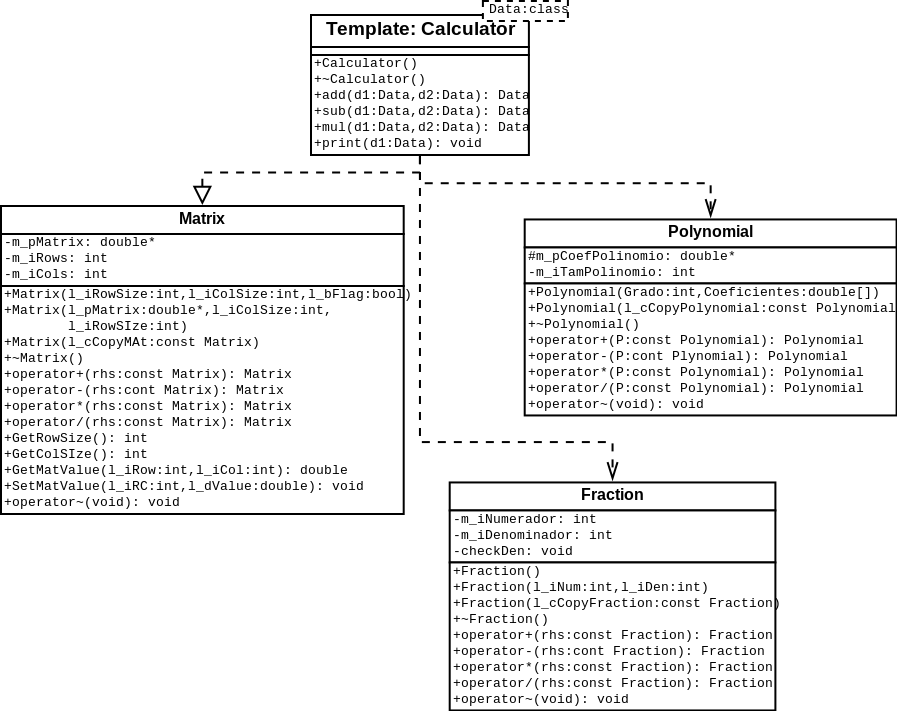
\includegraphics[width=\textwidth]{imgs/Labo4/Diagram2.png}
\caption{Diagrama UML.}
\label{fig:uml}
\end{figure}

%%%%%%%%%%%%%%%%%%%%%%%%%%%%%%%%%%%%%%%%%%%%%%%%%%%%%%%%%%%%%%
% --> RESULTADOS
%%%%%%%%%%%%%%%%%%%%%%%%%%%%%%%%%%%%%%%%%%%%%%%%%%%%%%%%%%%%%%
\section{Resultados}

A continuación se muestran los resultados de la implementación en el programa principal.

En la figura \ref{fig:res1}, se puede observar el resultado al ejecutar una prueba simple en el con las matrices. 

\begin{figure}[H]
\centering
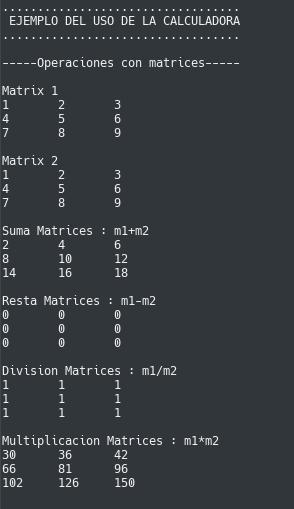
\includegraphics[width=.4\textwidth]{imgs/Labo4/result1}
\caption{Resultado de la implementación de la clase \texttt{Matrix}}
\label{fig:res1}
\end{figure}

Los resultados de la implementación de fracciones se muestran en la figura \ref{fig:res2}.

\begin{figure}[H]
\centering
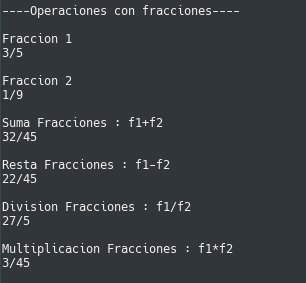
\includegraphics[width=.4\textwidth]{imgs/Labo4/result2}
\caption{Resultado de la implementación de la clase \texttt{Matrix}}
\label{fig:res2}
\end{figure}

Por último, en las figuras \ref{fig:res3} y \ref{fig:res4} se observa el resultado obtenido en el caso de las operaciones con polinomios.
\begin{figure}[H]
\centering
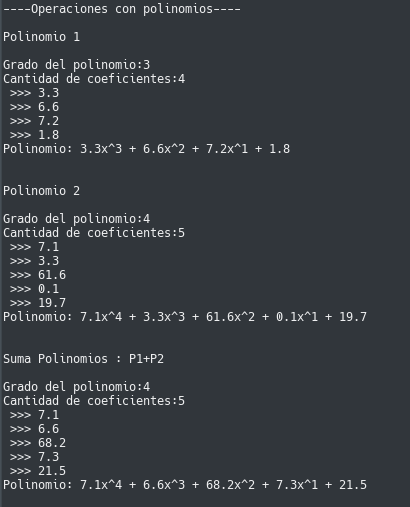
\includegraphics[width=.4\textwidth]{imgs/Labo4/result3}
\caption{Resultado de la implementación de la clase \texttt{Matrix}}
\label{fig:res3}
\end{figure}


\begin{figure}[H]
\centering
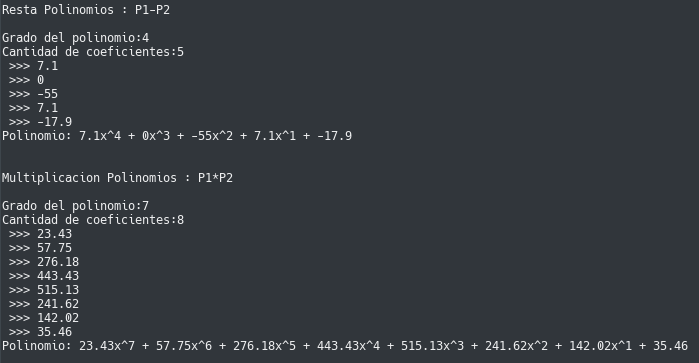
\includegraphics[width=.4\textwidth]{imgs/Labo4/result4}
\caption{Resultado de la implementación de la clase \texttt{Matrix}}
\label{fig:res4}
\end{figure}


%%%%%%%%%%%%%%%%%%%%%%%%%%%%%%%%%%%%%%%%%%%%%%%%%%%%%%%%%%%%%%
% --> CONCLUSIONES
%%%%%%%%%%%%%%%%%%%%%%%%%%%%%%%%%%%%%%%%%%%%%%%%%%%%%%%%%%%%%%
\section{Conclusiones}


Como conclusiones se tiene que:

\begin{itemize}
\item Se logra la implementación de las operaciones de suma, resta, multiplicación y división para diferentes tipos de datos matemáticos como lo son matrices, fracciones y polinomios por medio de la creación de clases para cada uno de estos datos.
\item Se implementa un operador para imprimir los datos según el tipo de información que se estaba manejando.
\item Se crea una clase emplantillada que logra llamar a las diferentes clases creadas y realizar las operaciones creadas.
\item Se comprende la utilidad del emplantillado de funciones y clases para la reutilización de código y orden del mismo.
\end{itemize}


%%%%%%%%%%%%%%%%%%%%%%%%%%%%%%%%%%%%%%%%%%%%%%%%%%%%%%%%%%%%%%
% --> BIBLIOGRAFIA
%%%%%%%%%%%%%%%%%%%%%%%%%%%%%%%%%%%%%%%%%%%%%%%%%%%%%%%%%%%%%%
\begin{thebibliography}{IEEE}
\bibitem{R1} Talens, S. \textbf{\textit{Curso de programación en C++}}. EUI (UPV) Valencia, 17 al 28 de Julio de 1995. 

\bibitem{R2} Raffo, E. \textbf{\textit{Programación genérica en C++, usando Metaprogramación}}. 2007. Sistemas de Informática. 
\end{thebibliography}
